\documentclass[a4paper,10pt]{article}

\usepackage{graphicx}
\graphicspath{{sections/images/}}
\usepackage{}
\usepackage{booktabs}
\usepackage{caption}
\usepackage[section]{placeins}
\usepackage{titlesec}

\usepackage{amsmath}
\usepackage{amsfonts}
\usepackage{amssymb}
\usepackage{hyperref}
\usepackage[a4paper, top=2cm, bottom=2cm, left=2.5cm, right=2.5cm]{geometry}

\setcounter{secnumdepth}{4}
\titleformat{\paragraph}
{\normalfont\normalsize\bfseries}{\theparagraph}{1em}{}
\titlespacing*{\paragraph}
{0pt}{3.25ex plus 1ex minus .2ex}{1.5ex plus .2ex}

\begin{document}
\begin{titlepage}
    \centering  
    \begin{figure}[ht]
        \centering
        
\includegraphics[width=\textwidth]{ise-logo.png}
    \end{figure}
    \vspace*{2cm} 
    
    {\Huge \textbf{Progress Report 1} \par}
    {\Huge \textit{Pookie: An AI-Driven Robot for Promoting Mental Well-being and Emotional Support} \par}
    \vspace{4cm}
    
    {\large \textbf{Authors:} Tibet Buramarn, Kridbhume Chammanard, and Thitaya Divari \par}
    \vspace{1cm}
    {\large \textbf{Advisor:} Dr. Paulo Fernando Rocha Garcia, Ph.D., Assistant Professor of AI and Robotics at Chulalongkorn University and \par}
    {\large Ms. Kunpariya Siripanit, Counseling Psychologist at Chula Student Wellness, Chulalongkorn University \par}

    \vspace{3cm}
    
    {\large 2147417 Final Project II \par}
    {\large International School of Engineering (ISE) \par}
    {\large Chulalongkorn University \par}
    
    \vspace{2cm}
    
    {\large February 28, 2025 \par}
    
    \vspace*{\fill}
\end{titlepage}

\thispagestyle{empty}

\newpage
\begin{center}
    \item\section*{Abstract}
\end{center}
\large
Pookie, an AI-driven robot for promoting mental well-being, developed under advisory with Chula Student Wellness, aims to create an AI-driven companion to enhance mental well-being by promoting positivity. The robot aims to address \textbf{\textit{“Terror Outbursts,”}} a future concern in Thailand involving an anxiety–driven society, where the robot aims to alleviate feelings of stress and anxiety by providing a feeling of slowness and emotional attachment. The robot integrates computer vision, feature extraction, sensors, and actuators to address key customer needs in appearance, interactivity, and empathy. The general appearance of the robot is an anthropomorphic design with resemblance to a bear, with sensors, motors, and screens to deliver personalized interactions to the user. 
\newpage
\begin{center}
    \item\section*{Acknowledgements}
\end{center}
The team expresses their sincere gratitude to Dr. Paulo Fernando Rocha Garcia, Ph.D., Assistant Professor of AI and Robotics at Chulalongkorn University, and Ms. Kunpariya Siripanit, Counseling Psychologist at Chula Student Wellness, Chulalongkorn University. Dr. Paulo’s expertise in artificial intelligence and robotics was instrumental in guiding the technical development of the emotional wellness robot, while Ms. Kunpariya’s insights into counseling psychology ensured the project’s alignment with mental health principles. The team also acknowledges the support provided by the faculty and staff of the International School of Engineering, whose assistance was invaluable throughout this project. 
\normalsize

\newpage
\tableofcontents

\newpage
\section{Introduction}
This progress report provides an update on the development of Pookie, an AI-driven robot designed to promote mental well-being, developed in assistance from Chula Student Wellness. Pookie aims to act as a companion to help alleviate feelings of stress and anxiety, especially in response to future societal concerns like "Terror Outbursts," an anxiety-driven phenomenon anticipated to affect Thailand. The project focuses on enhancing positivity and emotional attachment by creating a robot that interacts with users in an empathetic and calming manner.

\section{Overview}
As a quick recap for how Pookie works, the robot utilizes video and audio sensors to predict the user’s current facial and speech emotion. This is done through using convolutional neural networks for facial emotion recognition, and bidirectional LSTMs for speech emotion recognition. The robot processes the user’s inputs and determines the best interaction for the user. For instance, if the user seems to be down or sad, Pookie might choose to make a soft and calming sound, a cheerful face, and slow movements in order to emotionally engage with the user, supposedly attempting to empathize with the user. With that said, this section will provide an overview into Pookie’s implementation in semester 2, detailing what’s done, what’s being doing, and what needs to be done next.
\subsection{What’s done}
Overall, the team has finalized the overarching approach of the interaction with the robot. This process was not well defined in the last semester, which led to ambiguity towards the final presentation. To elaborate, it was not clear of what output the robot would elicit given a certain combination of emotions. If the user was sad, should the robot try to cheer the user up? Or should it maintain neutrality. As such, the team has decided to consult Chula Student Wellness again for a quick chat to obtain their thoughts on this problem. They told us that the factors going into determining the output were almost infinite, where even psychologists themselves have problems truly empathizing with a person, and determining what to do to make a person feel better. As such, they claim it is almost impossible for our project to empathize to that extent. Therefore, we settled on a more generalized approach, as shown in Figure \ref{fig:flow}.

\begin{figure}[ht]
    \centering
    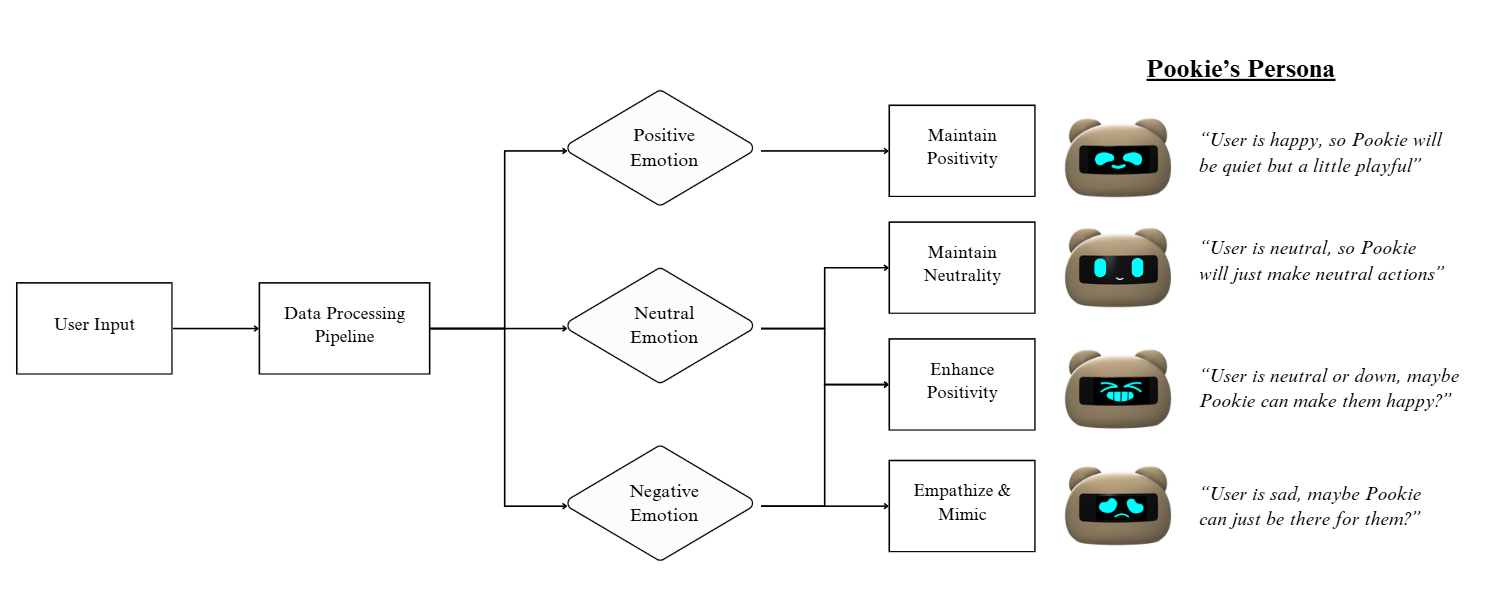
\includegraphics[width=\textwidth]{flow.png}
    \caption{Pookie Interaction Flowchart}
    \label{fig:flow}
\end{figure}

After processing inputs in the form of facial and speech emotion, the robot segments the output into 3 possible cases: positive, neutral and negative. With each case, the robot has a set of outputs it can perform. For instance, if the person is in a positive wellness state, Pookie will maintain positivity, meaning its intention will be to ensure this positive state of being of the user will be prolonged. On the other hand, if the user is neutral, Pookie will try to maintain this neutrality, but in some cases, such as if our models detect that the user is 60\% neutral, but 40\% happy, then the robot will elicit an output that could potentially make the user happier. Lastly, for the case of negative emotion, this part is tricky. The team has a design problem here: if the user is feeling negative, should the robot remain neutral? Should it show empathy? Or should it be fun and energetic? The underlying emotional factors, as we mentioned, are almost infinite, so we simplified it into two cases: either enhance positivity or empathize. In the case of empathy, the robot will simply mimic the user’s emotion (e.g sadness), with the intention of “being there” for the user. 

Another fundamental update is how Pookie processes the emotional inputs. Initially, the team finalized on the approach of finding the dominant emotion from the facial and speech emotion recognition models within a given time frame, then simply using those two dominant emotions to elicit an input. For instance, within 10 seconds, if a user made a “happy” face, and their speech is “happy”, then the output would be a positive maintenance. However, this approach disregarded many cases and made the robot very static. If the user’s face is “sad”, but their voice is “happy”, it’s impossible to combine these emotions and determine what the user’s true emotion is. This leads us to incorporating two new key technologies: bayesian networks and decision trees, creating a new flowchart as seen in Figure \ref{fig:rev_flow}.

\begin{figure}[ht]
    \centering
    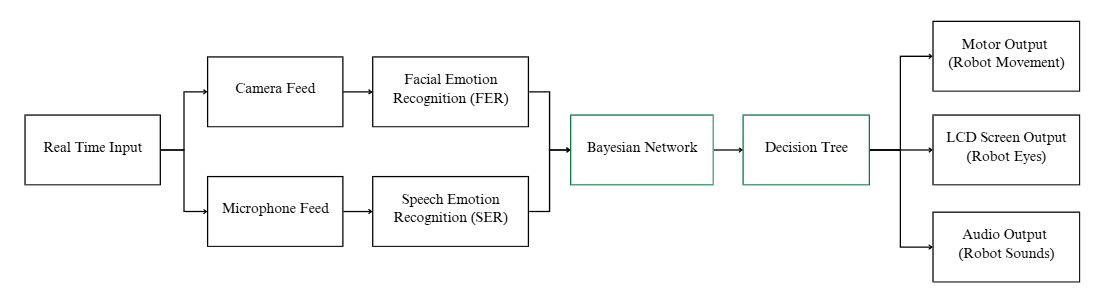
\includegraphics[width=\textwidth]{flow_revised.png}
    \caption{Revised Flowchart for Input Processing}
    \label{fig:rev_flow}
\end{figure}

The next update involves the implementation of the robot’s eyes, which is a fundamental interaction done through the LCD screen of the robot. Initially, the eyes of the robot used a Python library called OpenCV, which is an image processing library allowing the drawing of various shapes. The eyes were hard coded as various shapes and patterns drawn on a black canvas, as shown in Figure 3. The main challenge with this approach was the scalability and implementation time. Since each frame is hard coded, it does not allow for much flexibility and complex shapes. However, the upside is that it can easily be built in as a class into the main code. 

\begin{figure}[ht]
    \centering
    
\includegraphics[width=\textwidth]{happy.png}
    \caption{OpenCV Eyes Example for “Happy”}
    \label{fig:happy}
\end{figure}

The team decided on a different approach: using a simple software that could easily create dynamic shapes and record the frame sequence as a common file type, like GIF. The solution was Canva, a program typically used to make powerpoint slides, but with animation capabilities as well. Through implementing the eye sequence as a GIF format instead of hard coding, we are able to achieve more unique and personalized eye shapes and sequences for Pookie. Some examples of these are shown in Figure \ref{fig:new_eyes}.

\begin{figure}[ht]
    \centering
    
\includegraphics[width=\textwidth]{new_eyes.png}
    \caption{New Eyes Drawn as GIF Sequence on Canva}
    \label{fig:new_eyes}
\end{figure}

\newpage
Lastly, some other updates regard the hardware components. Our hardware team has completed a final design of Pookie in Fusion 360, and has acquired almost all necessary components needed for assembly. This will be discussed further in the hardware section.

\subsection{What we are working on}
This section discusses the currently ongoing tasks the team is working on this week and next week. Currently, the team is working on the Jetson Nano integration, which is the main processor for the project. Initially, in the last semester, the code, sensors, models, and so on were all hosted on a local computer, so it must be migrated and tuned so that it works appropriately with the Jetson Nano. Aside from this, we are working on coding the hardware functions, such as driving the servo motors, which are used to drive the arms, base, and neck of the robot. 

On the software side, although we have completed the Bayesian network, which is essential for predicting the user’s true emotion, the next part is also challenging: the decision tree. This requires the team to carefully design and process inputs. For instance, if the user is detected to be 50\% happy and 50\% sad at the same time, what does this constitute? Which set of actions should the robot perform: positive enhancement or maintenance. The team is working on carefully building this tree everyday, a few nodes at a time.


\newpage    
\section{Software}
\subsection{As-is Implementation}
The as-is data processing pipeline of Pookie is illustrated in Figure \ref{fig:flow-as-is}. In summary, the robot accepts real time inputs in the form of image frames and sound from its camera and microphone, then passes it through the facial and speech emotion recognition models respectively. Next, given a timeframe (e.g every 5 seconds), the models select the dominant emotion (i.e emotions with the highest confidence) then decide on the next best action based on that. For instance, if the dominant emotion from the FER and SER side are happy, then the output would be positivity maintenance. 

\begin{figure}[ht]
    \centering
    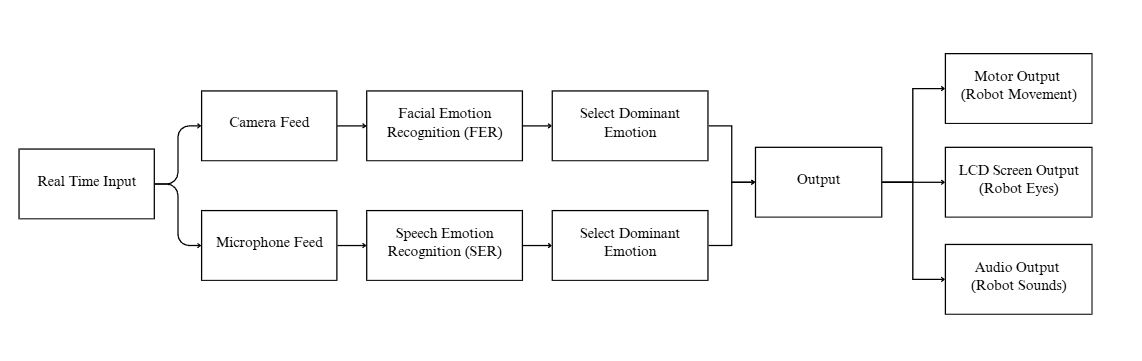
\includegraphics[width=\textwidth]{flow_as_is.png}
    \caption{Pookie As-is Implementation}
    \label{fig:flow-as-is}
\end{figure}

However, this design posed a few problems. Firstly, it does not take into consideration what the “true” emotion of the user is, which is fundamentally important. When people question what another person’s emotion is, they don’t look at the face and speech separately, but rather as one single emotion that captures what the person is feeling. We approached this problem by setting up a hypothesis of what the user could be feeling, then updating it with evidence from the FER and SER models, through using Bayesian Networks, which will be discussed in the next section. 

The next problem is ambiguity. Let’s say the output produced from FER and SER are 50\% happy and 50\% sad. With the initial approach, this case would be resolved using random selection, either sad or happy. However, this solution is quite ambiguous, and does not reflect realistic emotions. Thus, we decided to implement simplified decision trees, which use thresholds as a rule in navigating between nodes. The solution helps Pookie consistently navigate through complex or ambiguous emotions, but requires a lot of careful work in designing each node. This will be discussed in detail in the next section. 


\subsection{Challenges}
This section will discuss the challenges that were encountered during implementation. One major problem is the ambiguity of mapping of emotions. For context, each of the FER and SER emotions output a JSON of probabilities and their confidence (e.g Happiness 60\%, Neutral 30\%, Anger 10\%), with the potential outputs from each model shown in Table \ref{tab:emotion_mapping}. As shown in the figure, the models do not produce outputs with a 1:1 relationship, meaning some emotions from FER do not have a SER counterpart (such as FER output “Fear” does not have a corresponding emotion on the SER side). 

\begin{table}[h]
    \centering
    \begin{tabular}{|c|c|}
        \hline
        \textbf{Facial Emotion Recognition (FER) Outputs} & \textbf{Speech Emotion Recognition (SER) Outputs} \\
        \hline
        Neutral   & Neutral   \\
        \hline
        Anger     & Anger     \\
        \hline
        Happiness & Happiness \\
        \hline
        Sadness   & Sadness   \\
        \hline
        Disgust   & Frustration \\
        \hline
        Fear      & -         \\
        \hline
        Surprise  & -         \\
        \hline
    \end{tabular}
    \caption{Mapping of Emotions for SER and FER}
    \label{tab:emotion_mapping}
\end{table}

This inconsistency prevents the processing pipeline from functioning properly, necessitating the development of a solution. We have decided to map the missing speech emotion outputs to the most relevant existing speech emotions. While this approach may introduce some ambiguity, it provides a temporary fix for the emotion mapping issue. The newly mapped emotions are shown in Table \ref{tab:revised_mapping}.

\begin{table}[h]
    \centering
    \begin{tabular}{|c|c|}
        \hline
        \textbf{Facial Emotion Recognition (FER) Outputs} & \textbf{Speech Emotion Recognition (SER) Outputs} \\
        \hline
        Neutral   & Neutral   \\
        \hline
        Anger     & Anger     \\
        \hline
        Happiness & Happiness \\
        \hline
        Sadness   & Sadness   \\
        \hline
        Disgust   & Frustration \\
        \hline
        Fear      & Sadness (SER)   \\
        \hline
        Surprise  & Neutral (SER)   \\
        \hline
    \end{tabular}
    \caption{Revised Mapping of Emotions for SER and FER}
    \label{tab:revised_mapping}
\end{table}

In order to reduce the ambiguity caused by this substitution approach, we sought guidance from our advisor, Professor Paulo Garcia, who recommended exploring the Bayesian Network approach. The Bayesian Network approach will be discussed further in the next section.

\subsection{Revised Implementation using Bayesian Networks}

A Bayesian Network is a probabilistic graphical model that represents a set of variables and their conditional dependencies using a directed acyclic graph (DAG). It provides a structured approach to reasoning under uncertainty by encoding the probabilistic relationships between variables. In the context of Pookie, the Bayesian Network is used to infer the user's true emotional state by integrating evidence from both the FER and SER models.

The revised implementation introduces a Bayesian Network shown in Figure \ref{fig:bn}, where the user's underlying emotional state is treated as a latent variable, which is updated dynamically as new observations from FER and SER arrive. The network consists of nodes representing possible emotions and edges that define the probabilistic dependencies between them. Given an initial prior belief about the user's emotion, the system updates its belief by incorporating new observations from the FER and SER models using Bayes’ Theorem.

\begin{figure}[ht]
    \centering
    \includegraphics[width=\textwidth]{bn.png}
    \caption{Pookie's Bayesian Network}
    \label{fig:bn}
\end{figure}

\newpage
To construct the Bayesian Network, we defined conditional probability tables (CPTs) based on confusion matrices from both the FER and SER models seen in Figure \ref{fig:fer} and \ref{fig:ser} respectively, as well as insights from \textit{Emotions in Everyday Life} by Trampe et al. (2015) \cite{10.1371/journal.pone.0145450}, which provides probability distributions of emotions. By analyzing the confusion matrices, we estimated the likelihood of misclassifications and incorporated these probabilities into the CPTs, ensuring a more accurate representation of emotional relationships.

\begin{figure} [!ht]
    \centering
    \begin{minipage}{0.45\textwidth}
        \centering
        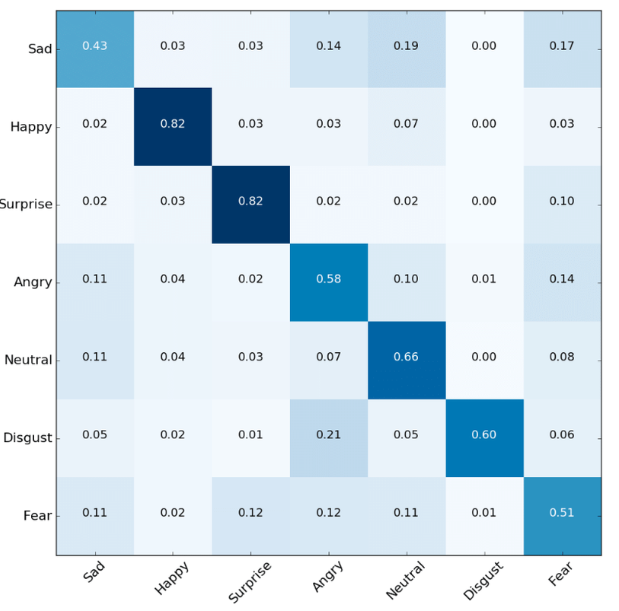
\includegraphics[width=\linewidth]{fer_confusion.png}
        \caption{FER Confusion Matrix}
        \label{fig:fer}
    \end{minipage}
    \hfill
    \begin{minipage}{0.45\textwidth}
        \centering
        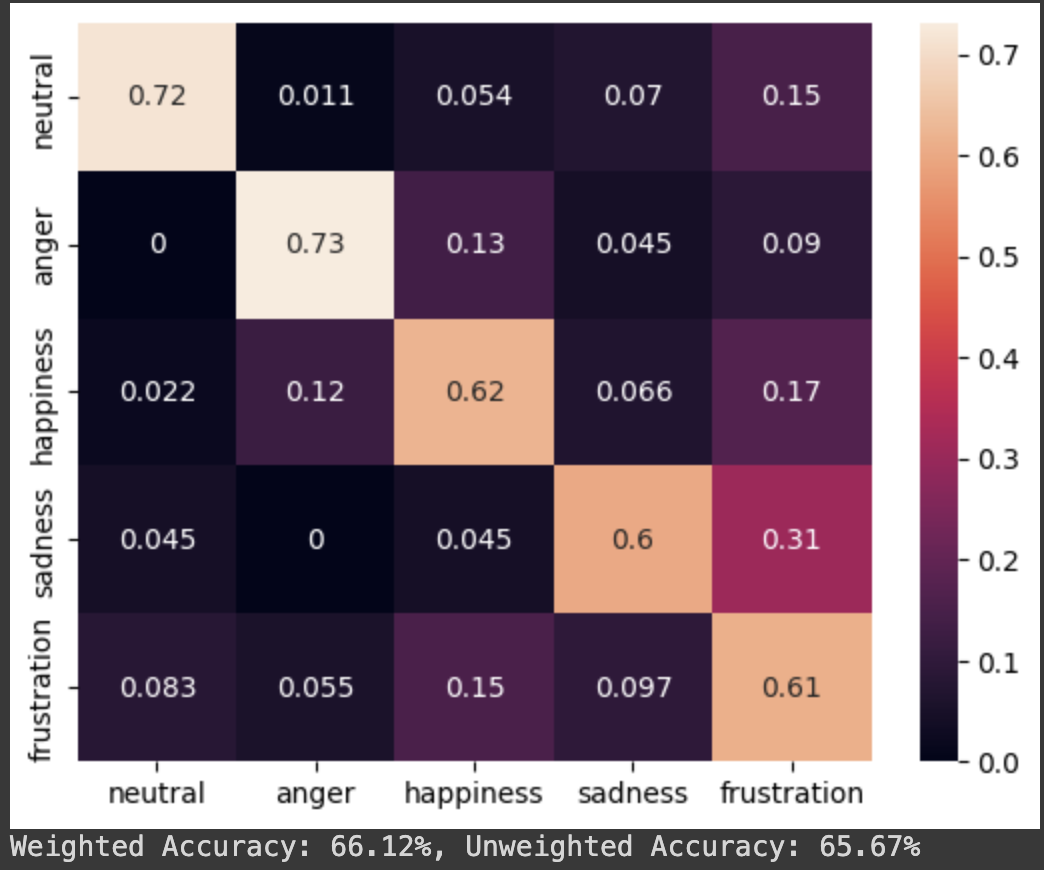
\includegraphics[width=\linewidth]{ser_confusion.png}
        \caption{SER Confusion Matrix}
        \label{fig:ser}
    \end{minipage}
\end{figure}

The confusion matrices represent how often the models correctly and incorrectly classify different emotional states. By utilizing these matrices, we were able to estimate the conditional probabilities for each emotional state. For example, if the FER model often misclassifies "Fear" as "Surprise" or "Sadness," these relationships are reflected in the CPTs. Similarly, if the SER model has a tendency to confuse "Frustration" with "Anger," the Bayesian Network accounts for these uncertainties when updating its belief about the user’s true emotion.

By combining the confusion matrix data with the probability distributions from the research paper, we constructed CPTs that better capture real-world emotional correlations. This approach allows the Bayesian Network to weigh the reliability of each model's predictions and adjust the estimated emotional state accordingly. Instead of treating FER and SER outputs as absolute truths, the system considers their likelihood of being correct based on historical performance.

To update the belief about the user’s emotional state, the Bayesian Network relies on Bayes’ Theorem, which provides a framework for calculating conditional probabilities. Specifically, the network uses the formula:

\[
P(E \mid R) = \frac{P(R \mid E) \cdot P(E)}{P(R)}
\]

Where:
\begin{itemize}
    \item \( P(E \mid R) \) is the posterior probability, representing the probability of the emotional state \( E \) given the result \( R \) (i.e., the FER and SER outputs).
    \item \( P(R \mid E) \) is the likelihood, which indicates how likely the result \( R \) is, given the emotional state \( E \).
    \item \( P(E) \) is the prior probability, representing the initial belief about the emotional state before observing the result, which is informed by the emotion distribution provided in \textit{Emotions in Everyday Life} by Trampe et al. (2015) \cite{10.1371/journal.pone.0145450}.
    \item \( P(R) \) is the evidence, or the total probability of observing the result under all possible emotional states.
\end{itemize}

In the context of Pookie, the emotional state \( E \) could be one of the possible emotions such as happiness, sadness, anger, etc. The result \( R \) is derived from the outputs of the FER and SER models, which provide a set of probabilities for each emotion. The likelihood \( P(R \mid E) \) is determined by the confusion matrices of the FER and SER models, which reflect how likely it is for the models to generate certain outputs given the true emotional state.

In this case, the likelihood \( P(R \mid E) \) is represented as the product of the probabilities from both the Facial Emotion Recognition (FER) and Speech Emotion Recognition (SER) models. Since we are dealing with two different models that provide independent estimates of the user’s emotional state, we combine these estimates by multiplying their corresponding probabilities for each emotion.

Thus, the likelihood for each possible emotional state \( E \) given the result \( R \) (which consists of the outputs from both the FER and SER models) can be expressed as:

\[
P(R \mid E) = P(R_{\text{FER}} \mid E) \cdot P(R_{\text{SER}} \mid E)
\]

Where:
\begin{itemize}
    \item \( P(R_{\text{FER}} \mid E) \) is the probability of the FER result \( R_{\text{FER}} \) given the emotional state \( E \).
    \item \( P(R_{\text{SER}} \mid E) \) is the probability of the SER result \( R_{\text{SER}} \) given the emotional state \( E \).
\end{itemize}

Since the FER and SER models are independent, their combined likelihood is simply the product of their individual likelihoods. This approach assumes that facial and speech expressions are conditionally independent given the true emotional state. By multiplying the probabilities, we take into account both the visual and auditory evidence of the user’s emotion, and use the combined evidence to estimate the true emotional state more accurately.

Thus, the updated Bayesian formula for computing the posterior probability of the emotional state \( E \) given the observations \( R_{\text{FER}} \) and \( R_{\text{SER}} \) becomes:

\[
P(E \mid R_{\text{FER}}, R_{\text{SER}}) = \frac{P(R_{\text{FER}} \mid E) \cdot P(R_{\text{SER}} \mid E) \cdot P(E)}{P(R_{\text{FER}}, R_{\text{SER}})}
\]

Where:
\begin{itemize}
    \item \( P(R_{\text{FER}}, R_{\text{SER}}) \) is the evidence or the total probability of observing both the FER and SER results. This is computed as the sum of the likelihoods over all possible emotional states:
\end{itemize}

\[
P(R_{\text{FER}}, R_{\text{SER}}) = \sum_{E} P(R_{\text{FER}} \mid E) \cdot P(R_{\text{SER}} \mid E) \cdot P(E)
\]

This formulation ensures that the system updates its belief about the user's emotional state by considering the likelihood of both the FER and SER outputs for each possible emotion. By combining the results from the facial and speech emotion recognition models, the Bayesian Network effectively integrates multiple sources of evidence, resulting in a more robust and accurate estimate of the user's true emotional state.

The use of multiplication for the likelihoods allows the Bayesian Network to properly account for the evidence from both modalities, reducing the impact of uncertainties and ambiguities from individual models. This approach improves the overall accuracy of the emotional assessment and enhances the robot's ability to make decisions that align with the user's true feelings.

The prior \( P(E) \) is based on a generalized distribution of emotional states, derived from external research, such as the findings from \cite{10.1371/journal.pone.0145450}. It reflects the average emotional distribution across a population and does not adjust based on an individual user’s history or context. This prior probability serves as a baseline, representing the general likelihood of each emotional state before any new observations from the FER and SER models are made.

Finally, \( P(R) \), the evidence, ensures that the posterior probabilities of all possible emotional states sum to 1. This value can be calculated as the sum of the likelihoods over all possible emotional states:

\[
P(R) = \sum_{E} P(R \mid E) \cdot P(E)
\]

By applying Bayes’ Theorem iteratively as new observations from the FER and SER models arrive, the Bayesian Network updates its belief about the user's emotional state. This update does not involve refining the estimate based on previous emotional history, but rather adjusts the system’s estimate by integrating the evidence from the two models in real time. This process allows the system to more accurately infer the user’s emotional state and navigate complex emotional situations with greater precision, reducing ambiguity and improving the overall user experience.

This probabilistic model enables Pookie to move beyond simple rule-based decision-making and handle the complexity of real-world emotional states more effectively.

\newpage
\section{Hardware}
This section details the hardware components and implementation of Pookie, illustrating the as-is design and the current design. Overall, the design concept has been finalized, and the team is working towards assembling and integrating all components. 

\subsection{Hardware Overview}
The 3D model of Pookie was created using Fusion 360, featuring a compact and interactive design. Initially, the design had a fully rounded head with a curved LED display, as shown in the earlier prototype in Figure \ref{fig:initial}. This design was akin to many referenced desktop robots, with a dynamic and engaging physical appearance. However, this was later modified because the LED screen is flat and does not conform to a curved surface. To accommodate this, the updated design features a more rectangular head with a flat front panel, ensuring proper integration of the LED display while still maintaining an anthropomorphic design. 

\begin{figure}[ht]
    \centering
    
\includegraphics[width=0.52\textwidth]{initial.png}
    \caption{Initial Design of Pookie}
    \label{fig:initial}
\end{figure}

Pookie’s LED display serves as its face, with illuminated eyes that create an engaging and friendly expression. Positioned above the display is a camera. Designed with a modularity concept, Pookie’s head and hands are detachable, allowing easy access to internal hardware for maintenance or upgrades. The spherical arms are designed to be movable, enhancing its interactive capabilities. The base of the robot houses the Jetson Nano, along with speakers for audio output. 

The design choices focus on creating a friendly, interactive, and easily maintainable robot, ensuring that Pookie remains both functional and engaging for users. In particular, the revisions made in semester 2 include modularity. For instance, Pookie’s head is not just a spherical helmet, but rather two half-spheres that can be assembled and disassembled. Additionally, Pookie’s arms and neck are now connected using a neodymium magnet, further contributing to its modular design. 

\begin{figure}[ht]
    \centering
    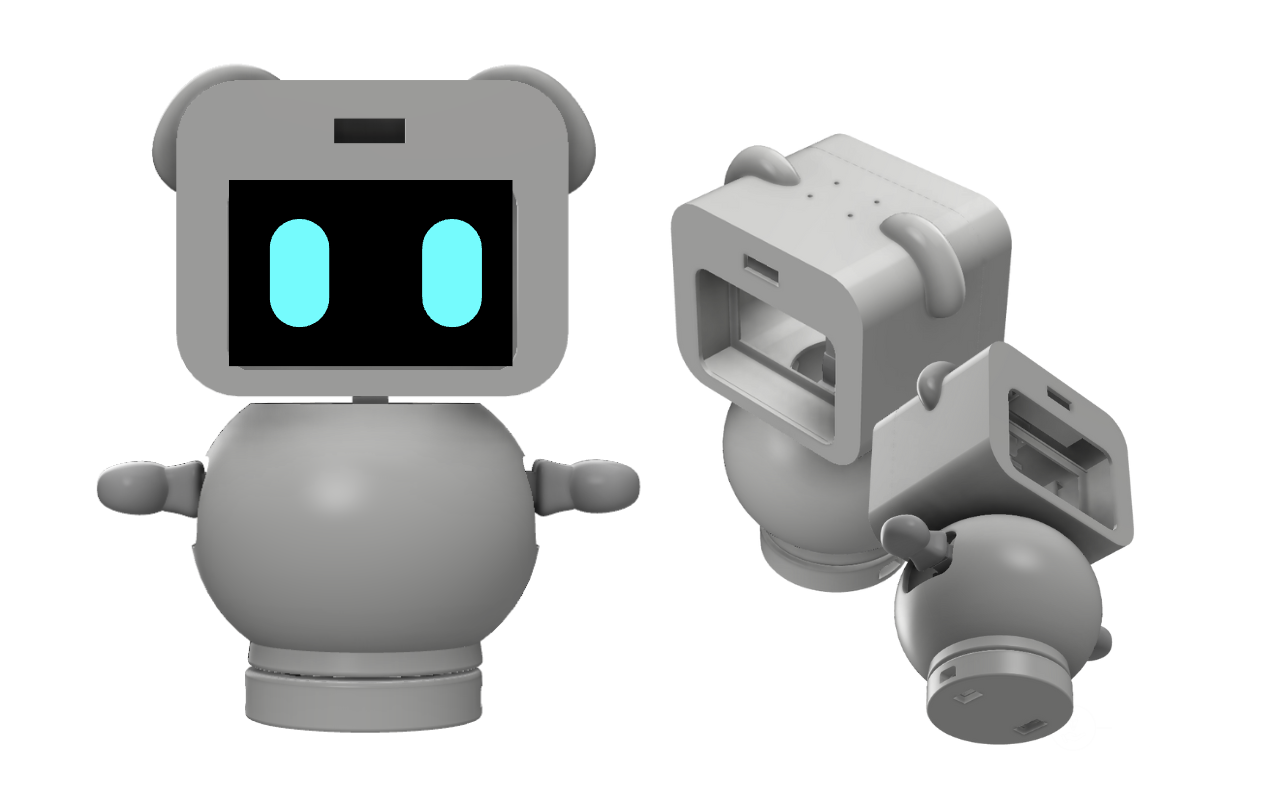
\includegraphics[width=0.85\textwidth]{new_des.png}
    \caption{Updated Design of Pookie}
    \label{fig:new_des}
\end{figure}

\newpage
Beneath the outer shell, Pookie's internal structure is designed to accommodate servo motors that control the movement of its head and arms by bevel gear mechanism allowing Pookie to perform simple gestures in a straightforward motion with four degrees of freedom. This is the as-is design, as shown in Figure \ref{fig:new_des}.

\begin{figure}[!ht]
    \centering
    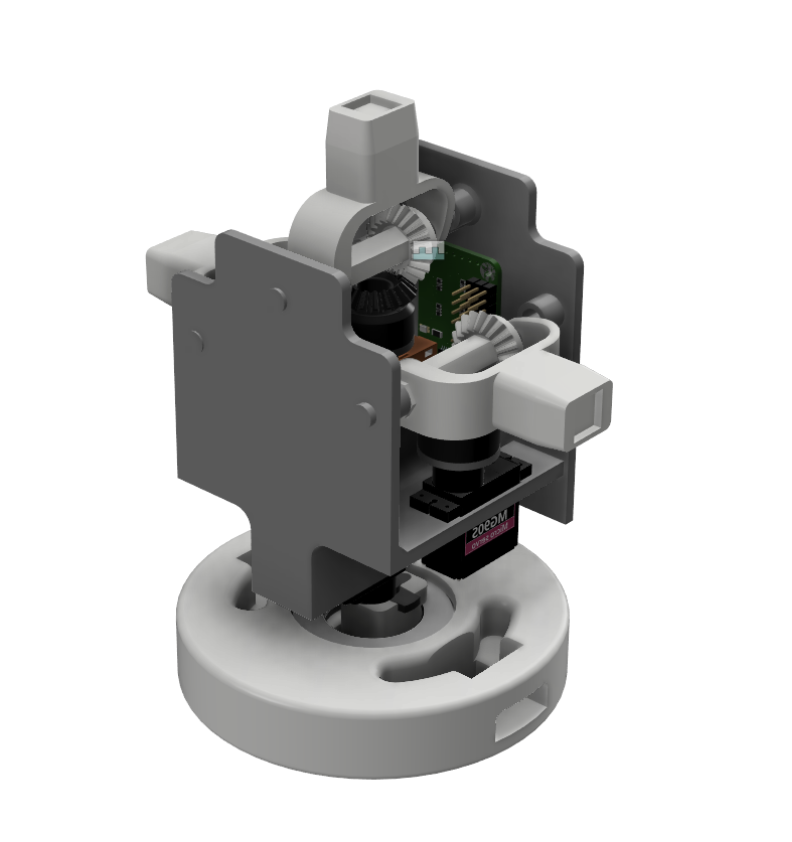
\includegraphics[width=0.6\textwidth]{internal.png}
    \caption{Internal Structure Design of Pookie}
    \label{fig:internal}
\end{figure}

Currently, several components of Pookie, including its head, motor brackets, gear, and other internal elements, have been 3D printed. Similarly, the hardware components necessary for assembly have almost all been acquired, missing only the speakers, which are rather hard to find. 

\subsection{Hardware Challenges}
One of the challenges encountered during the development process was ensuring that all 3D-printed components fit together properly. Some initial prints had slight misalignments, requiring adjustments to the design to achieve a more precise fit. These refinements helped improve the overall assembly process and ensure better compatibility between components.

Another challenge faced during the printing process was the size of each component, which was designed with flexibility in space in mind. This resulted in relatively large parts that could not fit in 3D printers. The solution was to break the parts into smaller pieces and construct them into one larger whole.


\newpage
\addcontentsline{toc}{section}{References}
\bibliographystyle{IEEEtran}
\bibliography{sections/references}

\end{document}
